\section{Problem Setup and Notation}

We first \fp{provide an review of} overview the Transition State Clustering algorithm.
\fp{we developed in CITE}

\subsection{Transition State Clustering Model}
At a high-level, the Transition State Clustering algorithm (\sys), clusters states that mark dynamical regime transitions across all demonstrations.
This finds a discrete parametrization for transition events that can be used for segmentation.
In our prior work, we found that this model was more robust in comparison to alternatives.\fp{such as X, Y, Z}
We first outline the model, and then describe the algorithm to fit the parameters.

\subsubsection{Dynamical System Model}
Let $\mathcal{D}=\{d_i\}$ \fp{$\mathcal{D}=\{d_1, \ldots, d_k\}$}be the set of demonstrations where each $d_i$ is a
trajectory $\mathbf{x}(t)=\binom{k(t)}{z(t)}$\fp{$\mathbf{x}:[0,1]\to \mathbb{R}^{a+b}$, $\mathbf{x}(t)=(k(t), v(t))$,
where $k(t)\in \mathbb{R}^a$ denotes kinematic and $v(t)\in \mathbb{R}^b$ visual features of ....} of fully observed robot states and each state is a vector in $\mathbb{R}^d$.
$\mathbf{x}(t)$ encapsulates both the kinematic state $k(t)$ and a set of visual features $z(t)$.
We model each demonstration as a switched linear dynamical system.
There is a finite set of $d \times d$ matrices $\{A_1,...,A_k\}$, and an i.i.d zero-mean additive Gaussian Markovian noise process $W(t)$ which accounts for noise in the dynamical model:
\[
\mathbf{x}(t+1) = A_{i}\mathbf{x}(t) + W(t) \text{ : } A_i \in \{A_1,...,A_k\}
\]
In this model, transitions between regimes are instantaneous where each time $t$ is associated with exactly one dynamical system matrix $1,...,k$.
\fp{notation: $i(t)\in \{1, \ldots, k\}$}

\subsubsection{Transition State Clusters}
\fp{A transition state is defined as the last state such that...}
Transition states are defined as the last states before a dynamical regime transition in \emph{each} demonstration.
Therefore, there will be times $t$ at which $A(t) \ne A(t+1)$.
A transition state is the state $x(t)$ at time $t$.
For a demonstration $i$, we denote the sequence of transitions states as $U_i=[u_i^1,...,u_i^J]$.
\fp{tuple notation typically uses round brackets $(u_i^1, \ldots, u_i^J)$.}
$J$ is the number of transition states where $J\ll T_i$ where $T_i$ is the time-length of $d_i$.

A \emph{transition state cluster} is
defined as a clustering of the set of transition states across all demonstrations; partitioning these transition states into $m$ non-overlapping similar groups:
\fp{reader might be lost here - do we have a simple image visualization of this process?}
\[
\mathcal{C} = \{C_1, C_2,...,C_m\}
\]
Every $U_i$ can be represented as a sequence of integers indicating that transition states assignment to one of the transition state clusters $U_i=[1,2,4,2]$.

We assume, demonstrations are \emph{consistent}, meaning there exists a non-empty sequence of transition states $\mathcal{U}^*$ such that the partial order defined by the elements in the sequence (i.e., $s_1$ happens before $s_2$ and $s_3$) is satisfied by every $U_i$. For example, 
\[U_1 = [1,3,4]\text{, }U_2 = [1,1,2,4]\text{, }\mathcal{U}^*=[1,4] \]
A counter example,
\[U_1 = [1,3,4]\text{, }U_2 = [2,5]\text{, }\mathcal{U}^*\text{  no solution} \]
Intuitively, this condition states that there have to be a consistent ordering of actions over all demonstrations up to some additional regimes (e.g., spurious actions). 
In case of multiple modes in an action sequence, we find the minimal consistent set.


\noindent \emph{Given a consistent set of demonstrations, the goal of the algorithm is to find a minimal solution, $\mathcal{U}^*$ that is loop free and respects the partial order of transitions in all demonstrations.}
\fp{Ken does not like cursive}
\subsection{Transition State Clustering Algorithm}

\begin{figure}[t!]
\centering
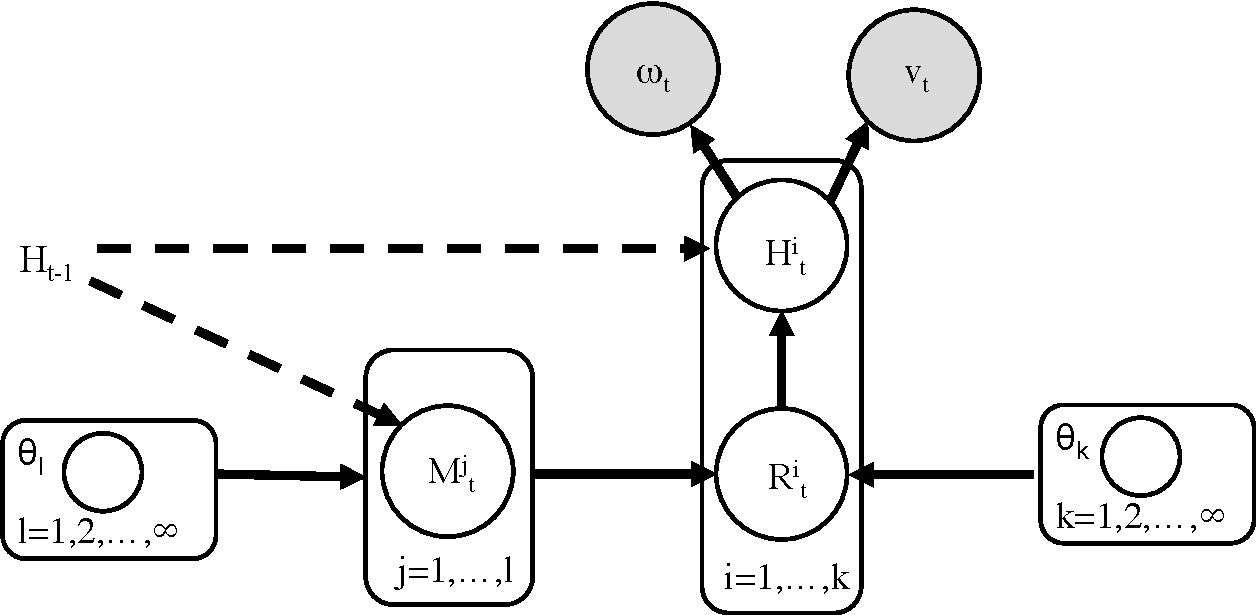
\includegraphics[width=\linewidth]{figures/pgm.pdf}
\caption{\todo{placeholder} (1) A finite-state Hidden Markov Chain with Gaussian Mixture Emissions (GMM+HMM) , and (2) TSC model. TSC uses Dirchilet Process Priors and the concept of transition states to learn a robust segmentation. }
\label{fig:tsc-pgm}
\vspace{-10pt}
\end{figure}


\subsubsection{Transition State Identification}
The first step is to identify a set of transition states for each demonstration in $\mathcal{D}$.
Suppose there was only one regime, then this would be a linear regression problem:
\[
\arg\min_A \|A X_t - X_{t+1}\|
\]
where $X_t$ is a matrix where each column vector is $x(t)$, and $X_{t+1}$ is a matrix where each column vector is the corresponding $x(t+1)$.
Moldovan et al. \cite{moldovan2013dirichlet} proves that fitting a Jointly Gaussian model to $n(t) = \binom{\mathbf{x}(t+1)}{\mathbf{x}(t)}$ 
\fp{stacked notation looks ugly}
is equivalent to Bayesian Linear Regression.
We use Dirichlet Process Gaussian Mixture Models to learn the regimes without have to set the number of regimes in advance.
Each cluster learned signifies a different regime, and co-linear states are in the same cluster.
To find transition states, we move along a trajectory from $t=1,...,t_f$, and find states at which $n(t)$ is in a different cluster than $n(t+1)$.
These points mark a transition between clusters (i.e., transition regimes).


\subsubsection{Transition State Clustering}\label{prun}
Each of these regimes will have constituent vectors where each $n(t)$ belongs to a demonstration $d_i$. 
Transition states that mark transitions to or from regimes whose constituent vectors come from fewer than a fraction $\rho$ demonstrations are \emph{pruned}.
$\rho$ should be set based on the expected rarity of outliers.

After pruning, there are numerous transition states at different locations in the state-space.
If we model the states at transition states as drawn from a GMM model:
\[
{x}(t) \sim N(\mu_i, \Sigma_i)
\]
Then, we can apply the DP-GMM again to cluster the state vectors at the transition states.
Each cluster defines an ellipsoidal region of the state-space space.
The result of the pruning and clustering is a set of transition state clusters.
\fp{overall this section is very long and a bit exhausting - we don't want the reader to be tired before getting into
    what's new. Maybe separating the comments on related work out into the related work section could help shorten the
algorithmic part?}
\subsection{Local Linearity of Visual Features}

\begin{figure}[t!]
\centering
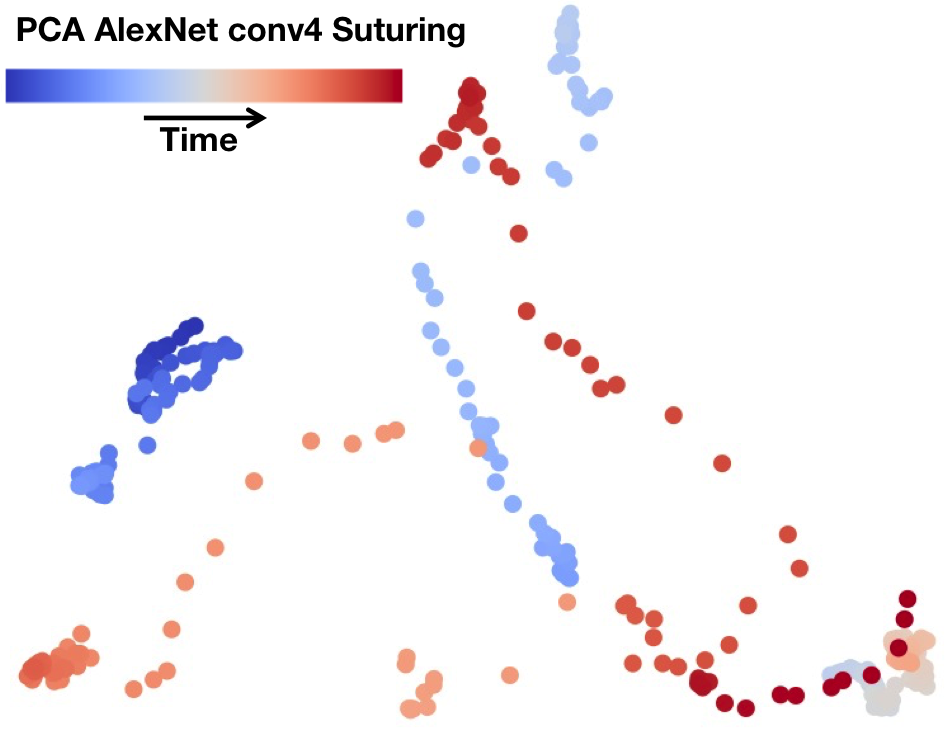
\includegraphics[width=0.7\linewidth]{figures/pca_conv4.png}
\caption{The figure visualizes the PCA projection of 64,896 dimensional output from \texttt{conv4} of the Alexnet for a sub-sequence of the suturing task video sub-sampled at 10 fps. The points are colored according to time from blue to red. We note that the visual features follow a smooth trajectory even in the high dimensional visual space.   \label{fig:imgtraj}}
\vspace{-10pt}
\end{figure}

We next describe why this model is still justified for the augmented state $\binom{k(t)}{z(t)}$.
\fp{make this much weaker - this still is a hypothesis, not a proven thing, move figure to experiments?}
In Figure \ref{fig:imgtraj}, for a single trajectory from one of our experimental datasets, we plot a 2D PCA visualization of the features from convolutional layer (\texttt{conv4}) of the pre-trained AlexNet architecture. We use a sub-sequence of the full task and sub-sample the data at 10 fps and for each frame, we add a point to the visualization, illustrating the trajectory in feature space. It is worth noting that the visual features follow a smooth trajectory even in the high dimensional visual space, supporting the assumptions of local linearity made by our model for identifying changepoints.
